\documentclass[]{book}

%These tell TeX which packages to use.
\usepackage{array,epsfig}
\usepackage{amsmath}
\usepackage{amsfonts}
\usepackage{amssymb}
\usepackage{amsxtra}
\usepackage{amsthm}
\usepackage{mathrsfs}
\usepackage{color}
\usepackage{graphicx}
\usepackage{bm}
\usepackage{tikz}
\usepackage{float}
%\usepackage{widthof}
\usetikzlibrary{arrows}

%Here I define some theorem styles and shortcut commands for symbols I use often
\theoremstyle{definition}
\newtheorem{defn}{Definition}
\newtheorem{thm}{Theorem}
\newtheorem{cor}{Corollary}
\newtheorem*{rmk}{Remark}
\newtheorem{lem}{Lemma}
\newtheorem*{joke}{Joke}
\newtheorem{ex}{Example}
\newtheorem*{soln}{Solution}
\newtheorem{prop}{Proposition}

\newcommand{\lra}{\longrightarrow}
\newcommand{\ra}{\rightarrow}
\newcommand{\surj}{\twoheadrightarrow}
\newcommand{\graph}{\mathrm{graph}}
\newcommand{\bb}[1]{\mathbb{#1}}
\newcommand{\Z}{\bb{Z}}
\newcommand{\Q}{\bb{Q}}
\newcommand{\R}{\bb{R}}
\newcommand{\C}{\bb{C}}
\newcommand{\N}{\bb{N}}
\newcommand{\M}{\mathbf{M}}
\newcommand{\m}{\mathbf{m}}
\newcommand{\MM}{\mathscr{M}}
\newcommand{\HH}{\mathscr{H}}
\newcommand{\Om}{\Omega}
\newcommand{\Ho}{\in\HH(\Om)}
\newcommand{\bd}{\partial}
\newcommand{\del}{\partial}
\newcommand{\bardel}{\overline\partial}
\newcommand{\textdf}[1]{\textbf{\textsf{#1}}\index{#1}}
\newcommand{\img}{\mathrm{img}}
\newcommand{\ip}[2]{\left\langle{#1},{#2}\right\rangle}
\newcommand{\inter}[1]{\mathrm{int}{#1}}
\newcommand{\exter}[1]{\mathrm{ext}{#1}}
\newcommand{\cl}[1]{\mathrm{cl}{#1}}
\newcommand{\ds}{\displaystyle}
\newcommand{\vol}{\mathrm{vol}}
\newcommand{\cnt}{\mathrm{ct}}
\newcommand{\osc}{\mathrm{osc}}
\newcommand{\LL}{\mathbf{L}}
\newcommand{\x}{\bm{x}}
\newcommand{\UU}{\mathbf{U}}
\newcommand{\support}{\mathrm{support}}
\newcommand{\AND}{\;\wedge\;}
\newcommand{\OR}{\;\vee\;}
\newcommand{\Oset}{\varnothing}
\newcommand{\st}{\ni}
\newcommand{\wh}{\widehat}

%Pagination stuff.
\setlength{\topmargin}{-.3 in}
\setlength{\oddsidemargin}{0in}
\setlength{\evensidemargin}{0in}
\setlength{\textheight}{9.in}
\setlength{\textwidth}{6.5in}
\pagestyle{empty}
\renewcommand{\thesection}{\arabic{section}}



\begin{document}

\begin{center}
{\Large Draft}\\
\textbf{Alireza Abrehforoush}\\ %You should put your name here
Date: 9-11-2022 %You should write the date here.
\end{center}
\vspace{0.2 cm}
%%%%%%%%%%%%%%%%%%%%%%%%%%%%%%%%%%%%%%%%%%%
\section{Upper bound for the recurrence relation}
\begin{equation}
\begin{split}
    t_c &= \left[2p\left(1-p\right)^3\right] \times \left( t_{c-1}+t_{c+1} \right) \\
    &+ \left[p^2\left(1-p\right)^2\right] \times \left( t_{c-2}+t_{c+2} \right) \\
    &+ \left[1-4p\left(1-p\right)^3-2p^2\left(1-p\right)^2\right] \times t_c \\
    &+ 1,  \quad c = 2,\ldots,n-4
\end{split}
\end{equation}
% Using the inequality $\left( 1 - p \right) \le e ^ {-p}$ we have:
% \begin{equation}
% \begin{split}
%     t_c &\le \frac{\left[2p e^{-3p}\right] \times \left( t_{c-1}+t_{c+1} \right) + \left[p^2 e^{-2p}\right] \times \left( t_{c-2}+t_{c+2} \right) + 1}{\left[4p\left(1-p\right)^3+2p^2\left(1-p\right)^2\right]} \\
%     &\le 
% \end{split}
% \end{equation}
Online solver suggests following closed form for the simplified form of our recurrence relation \\ ($t_c = x\left( t_{c-1} + t_{c+1} + t_{c-2} + t_{c+2} \right) + y$):
\begin{figure}[H]
    \centering
    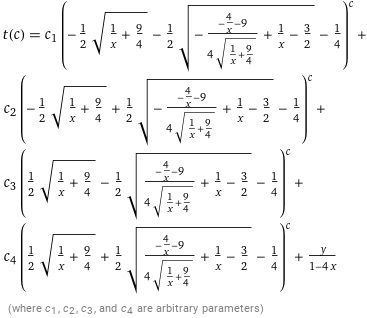
\includegraphics[width=0.7\textwidth]{figures/lower_bound.jpg}
    \caption{}
    %\label{fig:mesh2}
\end{figure}
We try to plot the abstract of each bases of the above exponential expressions (shifted down by 2).
\begin{equation}
\begin{split}
    y_1 &=\left| -\sqrt{\frac{1}{x}+\frac{9}{4}} - \sqrt{-\frac{-\frac{4}{x}-9}{4\sqrt{\frac{1}{x}+\frac{9}{4}}}+\frac{1}{x}-\frac{3}{2}} - \frac{1}{2} \right|-2 \\
    y_2 &=\left| -\sqrt{\frac{1}{x}+\frac{9}{4}} + \sqrt{-\frac{-\frac{4}{x}-9}{4\sqrt{\frac{1}{x}+\frac{9}{4}}}+\frac{1}{x}-\frac{3}{2}} - \frac{1}{2} \right|-2 \\
    y_3 &=\left| \sqrt{\frac{1}{x}+\frac{9}{4}} - \sqrt{\frac{-\frac{4}{x}-9}{4\sqrt{\frac{1}{x}+\frac{9}{4}}}+\frac{1}{x}-\frac{3}{2}} - \frac{1}{2} \right|-2 \\
    y_4 &=\left| \sqrt{\frac{1}{x}+\frac{9}{4}} + \sqrt{\frac{-\frac{4}{x}-9}{4\sqrt{\frac{1}{x}+\frac{9}{4}}}+\frac{1}{x}-\frac{3}{2}} - \frac{1}{2} \right|-2
\end{split}
\end{equation}
\begin{figure}[H]
    \centering
    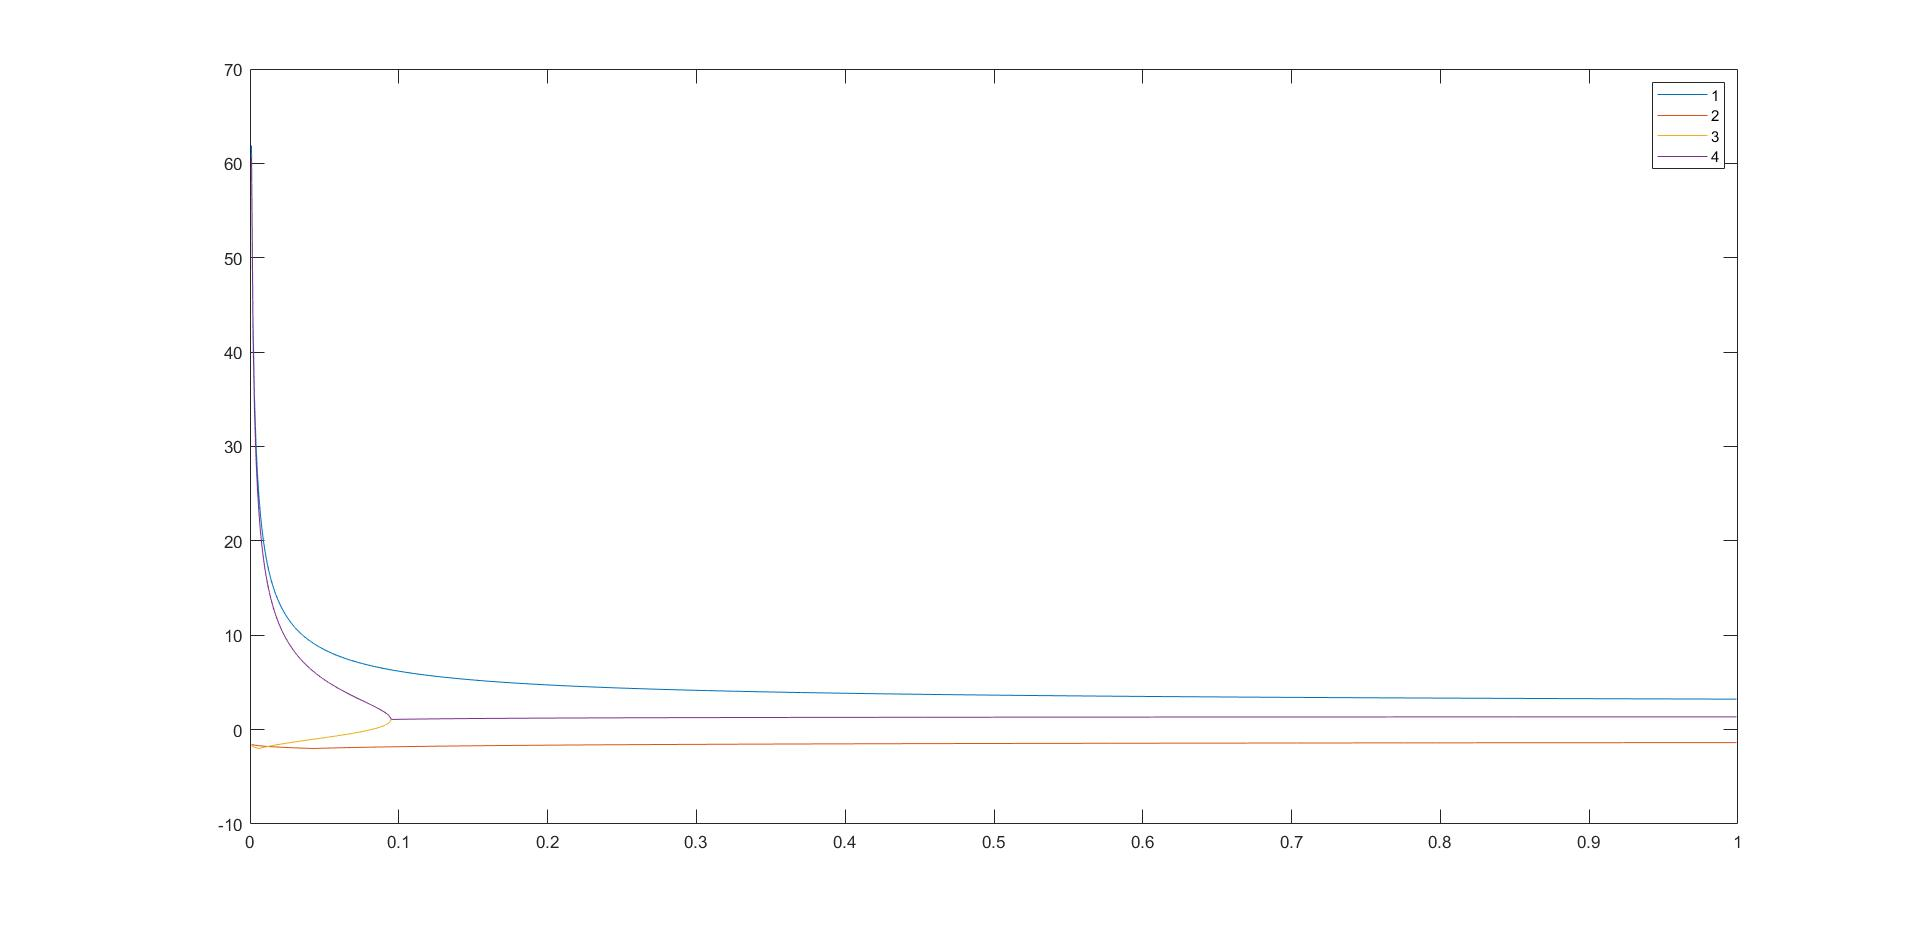
\includegraphics[width=1\textwidth]{figures/matfig1.jpg}
    \caption{}
    %\label{fig:mesh2}
\end{figure}
\begin{figure}[H]
    \centering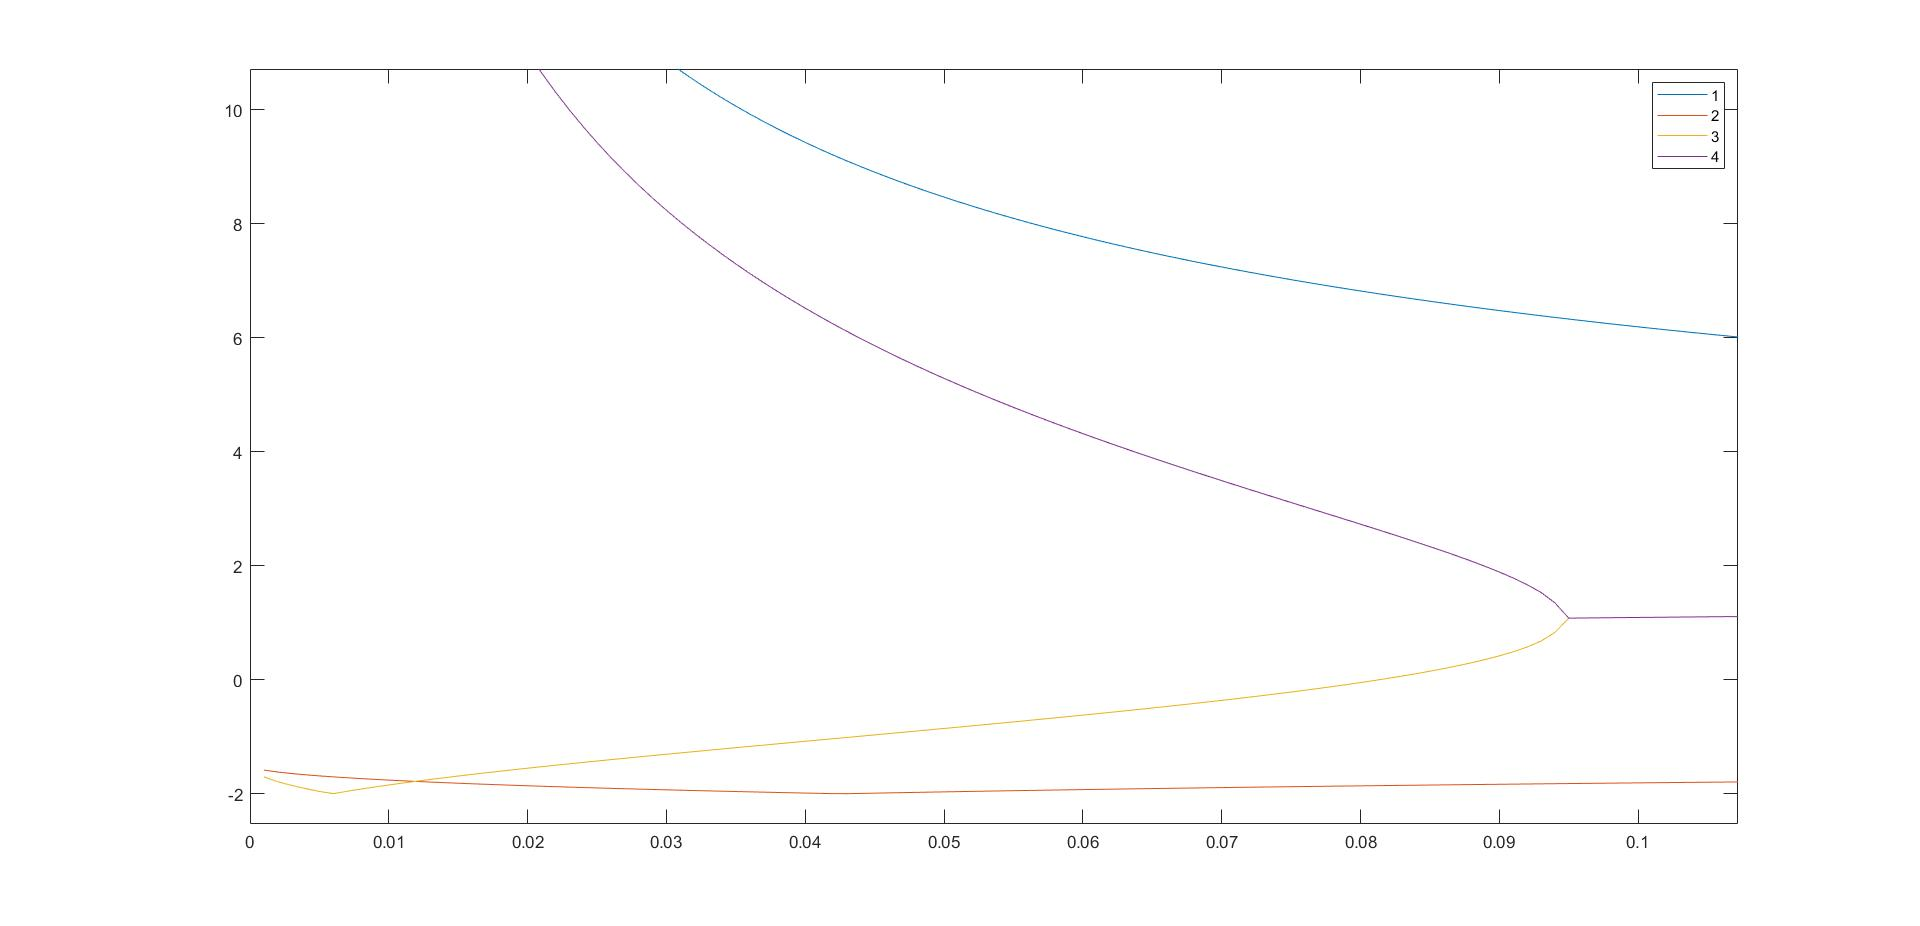
\includegraphics[width=1\textwidth]{figures/matfig2.jpg}
    \caption{}
    %\label{fig:mesh2}
\end{figure}

For $p \ge 1-p$ we can reach following lower bound:
\begin{equation}
\begin{split}
    t_c & \ge \frac{\left[ 1-p \right]^4 \times \left( t_{c-1} + t_{c+1} + t_{c-2} + t_{c+2} \right) + 1}{6p^4}
\end{split}
\end{equation}





\section{Matrix operations}


\section{Different transitions}
\subsection{Decomposition of an arc of length $k$ to two arcs of length $k_1$ and $k_2$}
\begin{figure}[H]
    \centering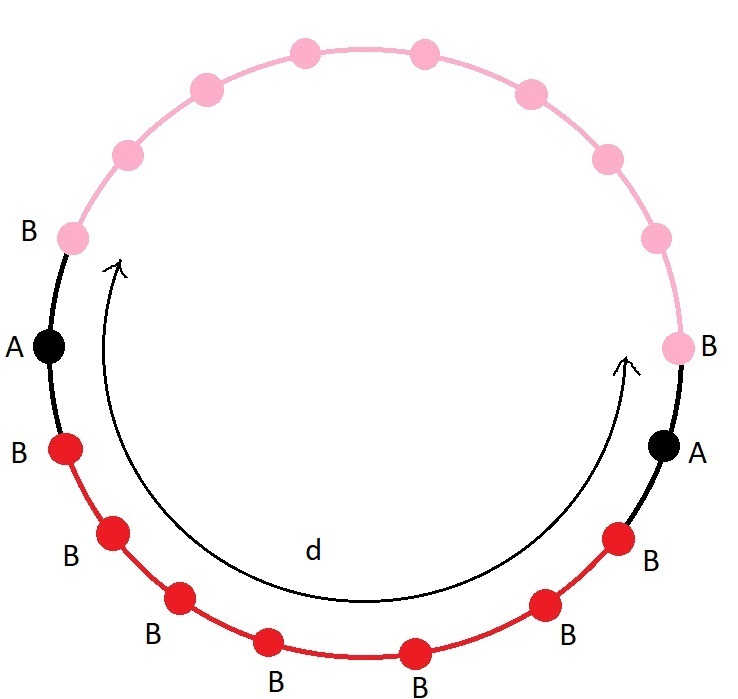
\includegraphics[width=0.4\textwidth]{figures/arc decomposition.jpg}
    \caption{}
    %\label{fig:mesh2}
\end{figure}
In any arbitrary configuration, transition can occur through decomposition of a red arc $X$ of length $k$ which is floating in a black region of length $d$ (i.e. the red arc in above figure) to two red arcs of length $k_1$ and $k_2$. The expected time to reach this system ($t_c$) is calculated as follows:
\begin{equation}
\begin{split}
    t_c &= \left[ p^k\left( 1-p \right) + p^{k_1}\left(1-p\right)^{k-k_1+1} + p^{k_2}\left(1-p\right)^{k-k_2+1} \right] \times 0 \\
    &+ p^k\left( 1-p \right) \times t_{c-1} \\
    &+ p^k\left( 1-p \right) \times t_{c+1} \\
    &+ \left[1 - 3p^k\left( 1-p \right) - p^{k_1}\left(1-p\right)^{k-k_1+1} - p^{k_2}\left(1-p\right)^{k-k_2+1} \right] \times t_c \\
    &+ 1, \quad c \in \left\{2, 3, \hdots, d-k-2 \right\}
\end{split}
\end{equation}
with following initial conditions:
\begin{equation}
\begin{split}
    t_1 &= p^k\left( 1-p \right) \times t_2 + \left( 1-p^k\left( 1-p \right) \right) \times t_1 + 1 \\
    t_{d-k-1} &= t_1
\end{split}
\end{equation}



\subsection{Sticking of two red arcs of lengths $k_1$ and $k_2$ respectively floating in a black region of length $d$ without reducing any red arc of length one ($k_1 + k_2 = k$)}
\begin{figure}[H]
    \centering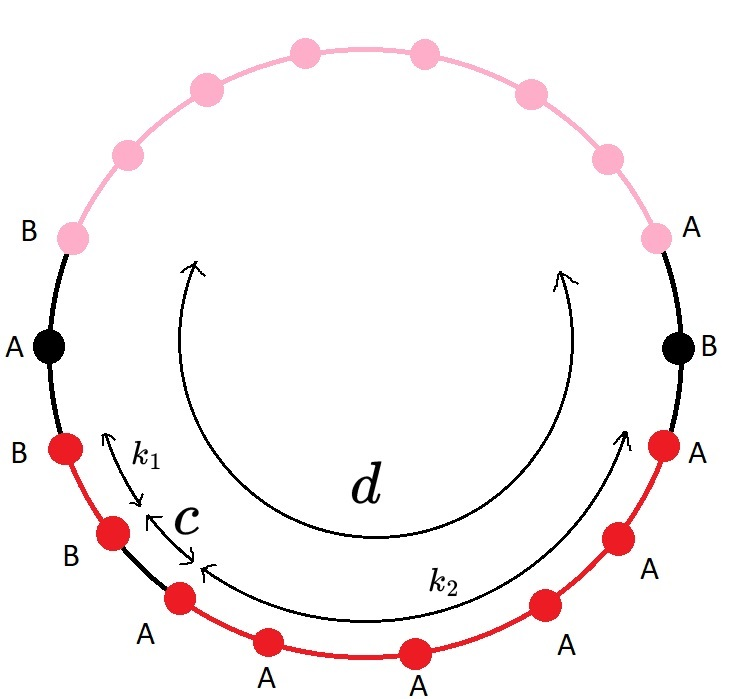
\includegraphics[width=0.4\textwidth]{figures/arcs sticking.jpg}
    \caption{}
    %\label{fig:mesh2}
\end{figure}

\begin{equation}
\begin{split}
    t_c &= \left[p^{k_1}\left( 1-p \right)^{k_2+2} + p^{k_2}\left( 1-p \right)^{k_1+2} \right] \times \left( t_{c-1} + t_{c+1} \right) \\
    &+ \left[ p^{k_1+k_2}\left( 1-p \right)^2 \right] \times \left( t_{c-2}+t_{c+2} \right) \\
    &+ \left[ 1 - 2p^{k_1}\left( 1-p \right)^{k_2+2} - 2p^{k_2}\left( 1-p \right)^{k_1+2} - 2p^{k_1+k_2}\left( 1-p \right)^2 \right] \times t_c \\
    &+ 1, \quad c \in \left\{ 3, 4, \hdots, d - k_1 - k_2 \right\}
\end{split}
\end{equation}
and following initial conditions:
\begin{equation}
\begin{split}
    t_0 &= 0 \\
    t_1 &= \left[p^{k_1}\left( 1-p \right)^{k_2+2} + p^{k_2}\left( 1-p \right)^{k_1+2} \right] \times \left( t_0 + t_2 \right) \\
    &+ \left[ p^{k_1+k_2}\left( 1-p \right)^2 \right] \times t_3 \\
    &+ \left[ 1 - 2p^{k_1}\left( 1-p \right)^{k_2+2} - 2p^{k_2}\left( 1-p \right)^{k_1+2} - p^{k_1+k_2}\left( 1-p \right)^2 \right] \times t_1 \\
    &+ 1
\end{split}
\end{equation}

\subsection{Increase of a red arc of length $k$ floating in a black region of length $d$ by two}
\begin{figure}[H]
    \centering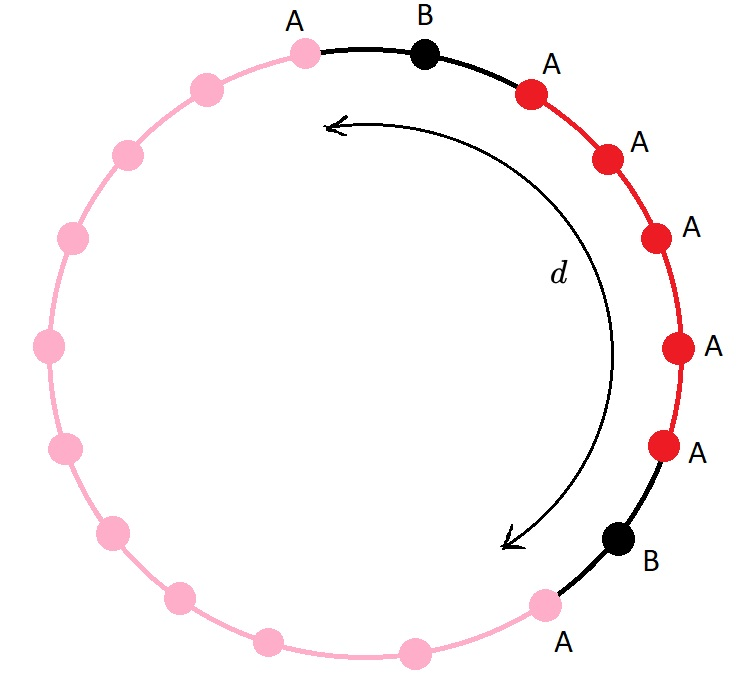
\includegraphics[width=0.4\textwidth]{figures/arc increase.jpg}
    \caption{}
\end{figure}

\begin{equation}
\begin{split}
    t_c &= \left[p^{k+1} \right] \times 0 \\
    &+ \left[ p^k\left( 1-p \right) \right] \times \left( t_{c-1} + t_{c+1} \right) \\
    &+ \left[1 - p^{k+1} - 2p^k\left( 1-p \right) \right] \times t_c \\
    &+ 1, \quad c \in \left\{ 2, 3, \hdots, d - k - 1 \right\}
\end{split}
\end{equation}
and following initial conditions:
\begin{equation}
\begin{split}
    t_1 &= \left[p^k\left( 1-p \right) \right] \times t_2 \\
    &+ \left[ 1 - p^k\left( 1-p \right) \right] \times t_1 \\
    &+ 1, \\
    t_{d-k-1} &= t_1
\end{split}
\end{equation}

\subsection{Disappearance of two red arcs}
\begin{figure}[H]
    \centering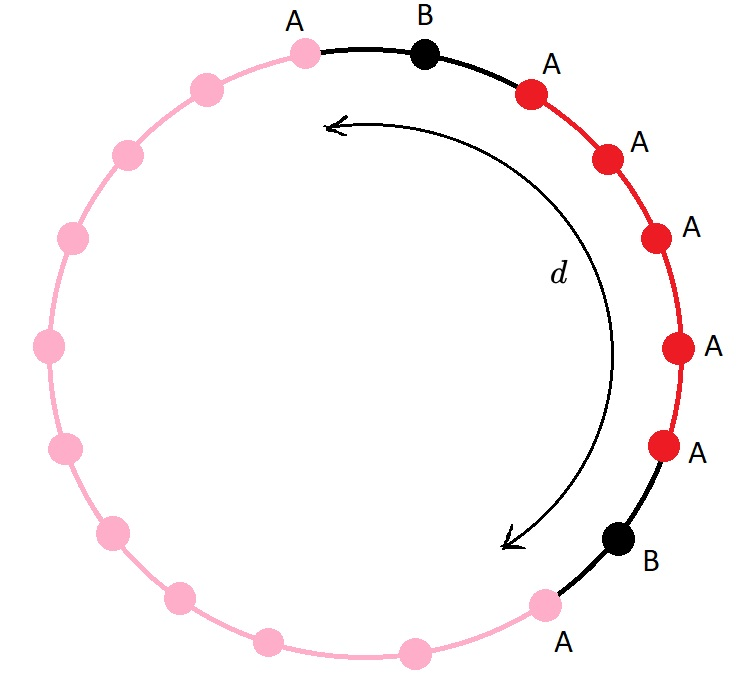
\includegraphics[width=0.4\textwidth]{figures/arc increase.jpg}
    \caption{}
\end{figure}


\end{document}